\begin{frame}
\frametitle{"Projet long" context}
\begin{block}{THC 2018 Challenge}
\begin{itemize}
\item Prepare tutorial challenge
\item Work based on \textit{GSMem: Data Exfiltration from Air-Gapped 
Computers over GSM Frequencies} (24th USENIX Security Symposium)
\item "Challenge" : data exfiltration form an air-gapped computer
\item "Tutorial" : guide the challenger step-by-step
\item Main idea : follow how we succeed to reproduce a part of the paper
\end{itemize}
\end{block}
\end{frame}

\begin{frame}
\frametitle{Air-gapped networks}
\centering 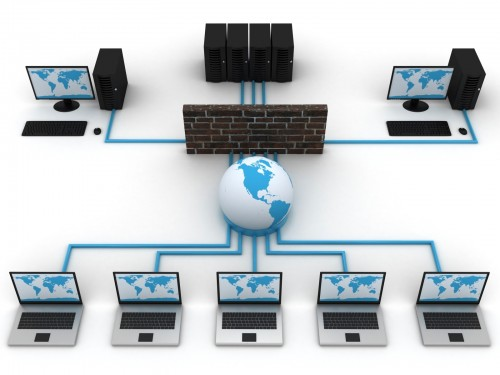
\includegraphics[scale=.5]{images/network.jpg}
\end{frame}

\begin{frame}
\frametitle{Air-gapped networks}
\centering 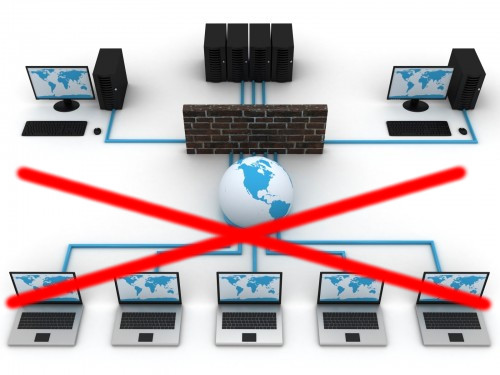
\includegraphics[scale=.5]{images/network2.jpg}
\end{frame}

\begin{frame}
\frametitle{Electromagnetic emanations}
\begin{block}{Emanations}
\begin{itemize}
\item Each electronic device has emanations
\item Could be electronical, acoustical, mecanical or electromagnetical
\item Focus on electromagnetic emanations
\end{itemize}
\end{block}

\begin{block}{TEMPEST}
\begin{itemize}
\item Name given by NSA for standards protecting against electromagnetic emanations
\item Context : EMSEC, surbpart of COMSEC
\end{itemize}
\end{block}
\end{frame}

\begin{frame}
\frametitle{Challenge context}
\begin{block}{Goal}
Get a password stored on the air-gapped computer
\end{block}

\begin{alertblock}{Problem}
Air-gapped computer $\Longrightarrow$ no possibility to gain access and/or exfiltrate data via network
\end{alertblock}

\begin{exampleblock}{Solution}
Use electromagnetic emanations to create a covert channel and exfiltrate data
\end{exampleblock}

\end{frame}


\begin{frame}
\frametitle{Technical environment}
\begin{block}{Devices}
\begin{itemize}
\item 1 air-gapped computer (attacked computer)
\item 1 standard computer (attacker's computer)
\end{itemize}
\end{block}

\begin{block}{Tools}
\begin{itemize}
\item Spectrum analyzer
\item Software-defined radio : USRP/RTL-SDR
\item Antennas
\item Softwares : URH/GNURadio
\end{itemize}
\end{block}



%\begin{center}
%
\includegraphics[scale=.37]{images/com.pdf}
%\end{center}
\end{frame}